\documentclass[dvipdfmx]{jsarticle}
\usepackage[dvipdfmx]{graphicx}
\usepackage{amsmath,amssymb,amsfonts,amsthm,enumerate}
\usepackage{float}
\usepackage{bm}
\usepackage{multirow}
\usepackage{hhline}
\usepackage{diagbox}
\usepackage{caption}
\usepackage{algorithm}
\usepackage{algpseudocode}
\usepackage{colortbl}
\usepackage[subrefformat=parens]{subcaption}
\captionsetup{compatibility=false}

\setlength\floatsep{0pt} %dblfloatsep

\newcommand{\argmax}{\mathop{\rm arg~max}\limits}
\newcommand{\argmin}{\mathop{\rm arg~min}\limits}

\newenvironment{hangall}[1]{\hangindent = #1zw\everypar{\hangindent = #1zw}}{}

\setlength{\topmargin}{-25mm}
\setlength{\textheight}{270mm}
\setlength{\oddsidemargin}{-10mm}
\setlength{\textwidth}{170mm}

\bibliographystyle{jplain}
\begin{document}

\begin{center}
  \begin {tabular}[h]{|c|c|c|c|c|c|c|c|}
  \multicolumn{8}{l}{}\\
  \hline
  \multicolumn{7}{|c|}{\begin{minipage}{120mm}\vspace{.2zh}TITLE\\[-3.1zh]\begin{center}
        %%%%%%%%%%%%%%%%%%%%%%%%%%%%%%%%%%%%%%%%%%
        提案手法とその具体例
        %%%%%%%%%%%%%%%%%%%%%%%%%%%%%%%%%%%%%%%%%%
      \end{center}\end{minipage}}
  &\begin{minipage}{20mm}Rep-No.\\[-.5zh]\hspace{3.5em}
    %%%%%%%%%%%%%%%%%%%%%
    2
    %%%%%%%%%%%%%%%%%%%
  \end{minipage}\\\hline
  \multicolumn{8}{|c|}{\begin{minipage}{120mm}\vspace{.2zh}AFFILIATION\\[-3.1zh]\begin{center}
        %%%%%%%%%%%%%%%%%%%%%%%%%%%%%%%%%%%%%%%%%%
        九州大学大学院 システム情報科学府 鈴木研究室
        %%%%%%%%%%%%%%%%%%%%%%%%%%%%%%%%%%%%%%%%%%
      \end{center}\end{minipage}}
  \\\hline
  \multicolumn{3}{|c}{\begin{minipage}{60mm}\vspace{.2zh}AUTHOR\\[-.7zh]
      \hspace{7em}Ichinose Haruki\end{minipage}}
  &\multicolumn{2}{|r}{\begin{minipage}{40mm}POSITION\\[-.7zh]\hspace{7.5em}B4\end{minipage}}
  &\multicolumn{3}{|c|}{\begin{minipage}{60mm}DATE\\[-.7zh]\hspace{9em}
      %%%%%%%%%%%%%%%%%%%%%%%%%%%%%%%%%%%%%
      2025/06/04
      %%%%%%%%%%%%%%%%%%%%%%%%%%%%%%%%%%%%%

    \end{minipage}}\\\hline
  \end{tabular}
\end{center}

\section{前回の発表について}
前回の発表では, データの偏見的説明に関する3つの先行研究の概要の説明を行った.
またそれらを踏まえ, 当初は新たな統計データから偏見的説明の生成を行う研究を提案していたが,
その後の検討により, 偏見的説明に対する対抗的な説明文を生成する研究へと方針を変更した.

\section{提案手法}

先行研究で示された偏見的説明の分類や, それらが悪用する人間的な本能の知見を活用し, LLMを用いて, 統計データとその偏見的説明文から, それに対する効果的な対抗説明文を生成する手法を提案する.
本提案手法は, 大きく分けて以下の2つのフェーズで構成する.
\begin{itemize}
  \item フェーズ1: SelectInstinctによる本能の特定
  \item フェーズ2: LLMによる対抗文生成
\end{itemize}

%%%%%%%%%%%%%%%%%%%%%%%%%%%%%%%%%%%%%%%%%%%%%%%%%%%%%%%%%%%%%%%%%%%%%%%%%%%%%%%%%

\subsection{フェーズ1: SelectInstinctによる本能の特定}
このフェーズでは, 偏見的説明文と関連する統計データから, その説明文が悪用している可能性の高い人間の本能を特定する.
その手法として, 先行研究で提案された偏見的説明文生成時の本能選択手続きであるSelectInstinctの考え方を使用する\cite{anonymous2024}.

\begin{figure}[H]
  \centering
  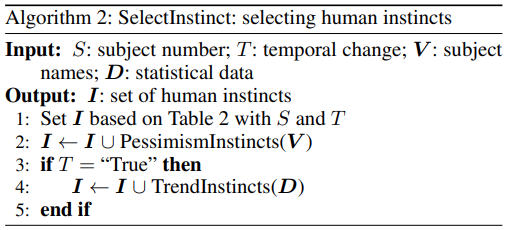
\includegraphics[width=0.5\textwidth]{01.png}
  \caption{SelectInstinct}
  \label{fig:selectinstinct}
\end{figure}

SelectInstinctは, 本来, 統計データの対象数S, 時間変化T, 対象名V, そして統計データDを分析し,
LLMが特定の偏見的説明文を生成するために, どの本能(例: 恐怖本能, ギャップ本能など)を悪用すべきかを自動で選択するアルゴリズム群として設計されている.

本フェーズでは, このSelectInstinctの「本能を選択する」というロジックを逆の視点から活用する. つまり, 偏見的説明文が,
どの本能を悪用することでその偏見を生み出しているのかを分析・特定するために, SelectInstinctの判断基準や手続きを指針として用いる.
\begin{itemize}
  \item \textbf{入力}
        \begin{itemize}
          \item S : 対象数
          \item T : 時間拡張の有無
          \item V : 変数名
          \item D : 統計データ
        \end{itemize}w3
  \item \textbf{出力}
        \begin{itemize}
          \item I : 偏見的説明文が悪用している可能性のある本能の集合
        \end{itemize}
\end{itemize}
%%%%%%%%%%%%%%%%%%%%%%%%%%%%%%%%%%%%%%%%%%%%%%%%%%%%%%%%%%%%%%%%%%%%%%%%%%%%%%%%

\subsection{フェーズ2: LLMによる戦略的対抗文生成}
このフェーズでは, フェーズ1で特定した情報に基づき, LLMを用いて対抗的な説明文を生成する.
プロンプトの主要構成要素: LLMに与えるプロンプトは, 主に以下の要素で構成する。
\begin{itemize}
  \item \textbf{入力}
        \begin{itemize}
          \item \textbf{統計データ}
          \item \textbf{偏見的説明文}
          \item \textbf{悪用している可能性のある本能の集合I}
          \item \textbf{対抗文生成のためのプロンプト:}
                \begin{itemize}
                  \item ペルソナ設計
                  \item Chain-of-Thought (CoT)を促す指示
                  \item 出力形式の指定
                \end{itemize}
        \end{itemize}
  \item \textbf{出力}
        \begin{itemize}
          \item \textbf{対抗文:} 偏見的説明文の誤りを指摘し, 統計データに基づいたより正確でバランスの取れた解釈を提示する説明文.
        \end{itemize}
\end{itemize}

%%%%%%%%%%%%%%%%%%%%%%%%%%%%%%%%%%%%%%%%%%%%%%%%%%%%%%%%%%%%%%%%%%%%%%%%%%%%%%%%

\section{具体例}

ここでは, 先行研究\cite{zhang2022,anonymous2024}で挙げられている
「Type V: 女性は男性よりも数学の点数が低い (Women have lower math scores than men.)」
を例に, 提案手法の適用イメージを示す.

\vspace{1em}

\begin{figure}[H]
  \centering
  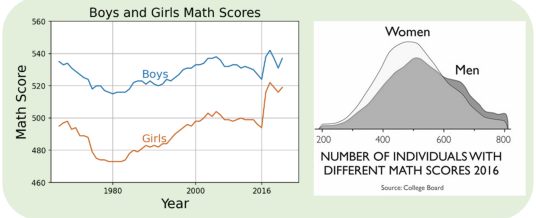
\includegraphics[width=0.5\textwidth]{02.png}
  \caption{Type V の統計データ(zhang2022\cite{zhang2022}より)}
  \label{fig:type_v_data}
\end{figure}

\vspace{1em}

\begin{itemize}
  \item \textbf{提示される情報:}
        \begin{itemize}
          \item 偏見的説明文: 「女性は男性よりも数学の点数が低い.」
          \item 統計データ: 男女別の数学の平均点の比較と, それぞれのスコア分布図.
        \end{itemize}

        \vspace{0.7em}

  \item \textbf{フェーズ1: SelectInstinctに基づく悪用されている本能の特定}
        \begin{itemize}
          \item 入力:
                \begin{itemize}
                  \item S : 2つ(男性と女性)
                  \item T : なし
                  \item V :「男性の数学の点数」「女性の数学の点数」
                  \item D : 男女の数学の平均点とスコア分布図(図\ref{fig:type_v_data}を参照)
                \end{itemize}
                \vspace{0.7em}

          \item 出力: \{分断本能, パターン化本能, ネガティブ本能, 単純化本能\}
        \end{itemize}

        \vspace{0.7em}

  \item \textbf{フェーズ2: LLMによる対抗文生成}
        \begin{itemize}
          \item プロンプトの構成要素:
                \begin{itemize}
                  \item \textbf{統計データ:} 男女の数学の平均点とスコア分布図.
                  \item \textbf{偏見的説明文:} 「女性は男性よりも数学の点数が低い.」
                  \item \textbf{特定された本能:} \{分断本能, パターン化本能, ネガティブ本能, 単純化本能\}
                  \item \textbf{ペルソナ設計:}\\
                        「あなたはデータリテラシーの専門家です. 統計データの誤解を解き, より正確でバランスの取れた理解を促すことを目指しています.」
                  \item \textbf{Chain-of-Thought (CoT)を促す指示:}
                        \begin{enumerate}
                          \item 偏見的説明文が悪用している特定の本能を分析する.
                          \item 偏見を正し, 客観的な事実を伝える対抗説明文を生成する.
                        \end{enumerate}
                  \item \textbf{出力形式の指定:} 簡潔で分かりやすい説明.
                \end{itemize}
                \vspace{0.7em}

          \item \textbf{期待される出力:}\\
                「平均点だけを見ると女性は男性よりも数学の点数が低いと感じるかもしれませんが, スコア全体の分布図に注目すると, 実際には男女のスコアは広範囲に重なり合っています.
                高い点数の女性も, 低い点数の男性も多く存在するため, 性別だけで数学の能力を一般化することは, データの全体像を見誤る可能性があります.」
        \end{itemize}
\end{itemize}

%%%%%%%%%%%%%%%%%%%%%%%%%%%%%%%%%%%%%%%%%%%%%%%%%%%%%%%%%%%%%%%%%%%%%%%%%%%%%%%%%

\begin{thebibliography}{99}
  \bibitem{zhang2022}
  K. Zhang, H. Shinden, T. Mutsuro, and E. Suzuki. Judging Instinct Exploitation in Statistical Data Explanations Based on Word Embedding. In \textit{Proc. AIES ’22}, pp. 867–879, 2022.

  \bibitem{anonymous2024}
  Anonymous. Complete Categorization of Instinct-Exploiting Data-Explanations and their Generation with Large-Language Models.

\end{thebibliography}
\end{document}